\documentclass{article}

% NeurIPS style -- download neurips_2026.sty from the NeurIPS website
% or use: \usepackage[margin=1in]{geometry} as a fallback
\IfFileExists{neurips_2026.sty}{
  \usepackage[final]{neurips_2026}
}{
  \usepackage[margin=1in]{geometry}
  \usepackage{times}
}

\usepackage[utf8]{inputenc}
\usepackage[T1]{fontenc}
\usepackage{hyperref}
\usepackage{url}
\usepackage{booktabs}
\usepackage{amsfonts}
\usepackage{amsmath}
\usepackage{amssymb}
\usepackage{nicefrac}
\usepackage{microtype}
\usepackage{xcolor}
\usepackage{pgfplots}
\usepackage{pgfplotstable}
\usepackage{subcaption}
\usepackage{algorithm}
\usepackage{algorithmic}
\usepackage{tikz}
\usetikzlibrary{arrows.meta, positioning, shapes.geometric, fit, calc}

\pgfplotsset{compat=1.18}

\title{Neural Conjecture Generation for Automated Theorem Proving\\via Symbol-Anonymous Graph Neural Networks}

\author{%
  Anonymous Authors\\
  \texttt{anonymous@example.com}
}

\begin{document}

\maketitle

\begin{abstract}
We present a neural system for generating useful intermediate lemmas (``cuts'')
that speed up automated theorem provers. Given a first-order logic problem in
clausal normal form (CNF), our system encodes it as a heterogeneous graph using
a graph neural network with an optional \emph{named symbol embedding} layer---where
well-known Mizar library symbols receive learnable embeddings while problem-specific
Skolem symbols remain fully anonymous. A pointer-based autoregressive decoder then
generates candidate lemmas by selecting symbols from the encoded graph. We introduce
\emph{arity-constrained decoding}, a generation-time technique that enforces
syntactic validity without retraining, improving validity from 2\% to 85--88\%.
We systematically compare eight model configurations across five decoder architectures
(Transformer, SSM/Mamba-style, conditional VAE, graph growing, and subgraph completion)
on the Mizar40 dataset of 3,161 problems with 122,356 labeled cuts, using a proper
train/validation/test split of 2,239/279/279 problems. Named symbol embeddings
reduce validation loss from 0.474 to 0.289 (best configuration). On 279 held-out
test problems, the best model generates conjectures of which 61\% are provably
correct lemmas and 5.8\% provide actual proof speedups, with the best achieving a
\textbf{77$\times$ reduction} in proof search. These results demonstrate that
combining structural graph representations with targeted symbol semantics yields
effective conjecturing strategies that generalize to unseen mathematical theories.
\end{abstract}

%==============================================================================
\section{Introduction}
\label{sec:intro}
%==============================================================================

Automated theorem provers (ATPs) such as E~\cite{schulz2002ebrainiac},
Vampire~\cite{kovacs2013vampire}, and SPASS~\cite{weidenbach2001spass}
search for proofs by systematically exploring the space of logical inferences.
For hard problems, this search can require processing thousands or millions
of clauses. A well-chosen intermediate lemma---a \emph{cut}---can dramatically
reduce this search by decomposing a hard problem into two easier subproblems.

Finding good cuts traditionally requires either human mathematical insight or
expensive enumeration. Recent work has explored using machine learning to guide
proof search~\cite{jakubuv2017enigma,loos2017deep,bansal2019holist}, but
\emph{generating} novel intermediate lemmas remains largely unexplored.

We address this challenge with a neural system that:
\begin{enumerate}
\item Encodes CNF problems as heterogeneous graphs with a \textbf{GNN encoder}
      supporting both fully symbol-anonymous and hybrid named-embedding modes;
\item Introduces \textbf{named symbol embeddings} for ${\sim}3{,}097$ Mizar
      library symbols while keeping Skolem symbols anonymous, reducing validation
      loss from 0.474 to 0.289;
\item Generates candidate lemmas via a \textbf{pointer-based autoregressive
      decoder} that selects symbols directly from the encoded graph;
\item Enforces syntactic validity through \textbf{arity-constrained decoding},
      a generation-time state machine requiring no retraining;
\item Achieves \textbf{61\% provability rate} on test-set conjectures,
      \textbf{5.8\% useful speedup rate}, and up to \textbf{77$\times$ proof speedup}.
\end{enumerate}

Our key finding is that combining structural anonymity with targeted name-based
priors yields the best results: the model achieves 98\% symbol precision in anonymous
mode (almost never generating symbols absent from the problem), and named embeddings
further improve the quality of generated conjectures across all three competitive
decoder architectures. Surprisingly, validation loss does not predict test-set
usefulness: the model with the worst validation loss among named configurations
(D+named, 0.413) achieves the best test useful rate (5.8\%), revealing a fundamental
exploration--exploitation trade-off in conjecture generation.

%==============================================================================
\section{Related Work}
\label{sec:related}
%==============================================================================

\paragraph{Machine learning for theorem proving.}
ENIGMA~\cite{jakubuv2017enigma} uses gradient-boosted trees to select given
clauses in saturation-based provers. DeepMath~\cite{alemi2016deepmath} and
FormulaNet~\cite{wang2017formulanet} learn premise selection for theorem proving.
HOList~\cite{bansal2019holist} applies reinforcement learning to interactive
theorem proving. GraphSAGE-based approaches~\cite{paliwal2020graph} encode
formulas as graphs for premise selection. Our work differs in \emph{generating}
novel lemmas rather than selecting from existing ones.

\paragraph{Conjecture generation.}
TerpreT~\cite{gauthier2021tactictoe} and related work explore conjecture synthesis
in interactive provers. The INT system~\cite{wu2021int} generates synthetic
theorems for curriculum learning. Most prior work operates on higher-level
representations; we work directly with first-order CNF clauses at the prover level.

\paragraph{Graph neural networks for logic.}
GNNs have been applied to SAT solving~\cite{selsam2019learning}, formula
classification~\cite{crouse2019improving}, and premise selection~\cite{paliwal2020graph}.
Our heterogeneous graph representation with 5 node types and 16 edge types is
specifically designed for the rich structure of first-order CNF clauses.

\paragraph{Pointer networks.}
Pointer networks~\cite{vinyals2015pointer} select from variable-size input
vocabularies, which is essential when the output must reference symbols from
the specific input problem. Our decoder extends this with structured tree generation.

%==============================================================================
\section{Problem Formulation}
\label{sec:problem}
%==============================================================================

\subsection{CNF Problems and Cuts}

A CNF problem $P$ consists of clauses $C_1, \ldots, C_n$, where each clause
$C_i = l_1 \lor l_2 \lor \cdots \lor l_m$ is a disjunction of literals. Each literal
is a possibly-negated predicate applied to terms, which may be variables (universally
quantified), constants, or function applications.

Given a candidate lemma $C$ (itself a CNF clause), we define the \emph{cut evaluation}:
\begin{itemize}
\item \textbf{P1}: Prove $P$ with $C$ added as an axiom (does $C$ help?)
\item \textbf{P2}: Prove $C$ from $P$ by refuting $P \cup \{\neg C\}$ (is $C$ valid?)
\end{itemize}

If both succeed with proof search lengths $L_1$ and $L_2$ respectively, the
\emph{speedup ratio} is $r = (L_1 + L_2) / L$, where $L$ is the original proof
search length. A ratio $r < 1$ indicates a useful cut.

\subsection{Dataset}

We use the Mizar40 cut dataset~\cite{kaliszyk2015mizar40}, consisting of 3,161 CNF
problems with 122,356 evaluated cuts (Table~\ref{tab:dataset}). Each cut is a clause
extracted from E prover's proof, with a measured speedup ratio.

\begin{table}[t]
\centering
\caption{Dataset statistics.}
\label{tab:dataset}
\begin{tabular}{lr}
\toprule
\textbf{Metric} & \textbf{Value} \\
\midrule
Total problems & 3,161 \\
Total evaluated cuts & 122,356 \\
Good cuts ($r < 1.0$) & 44,895 (36.7\%) \\
Excellent cuts ($r < 0.1$) & 1,509 (1.2\%) \\
Unique Mizar symbols & 5,105 \\
Unique Skolem patterns & 305 \\
Median graph nodes per problem & 395 \\
\bottomrule
\end{tabular}
\end{table}

We split by \emph{problem} (not by cut) to prevent data leakage:
2,239 problems for training (80\%), 279 for validation (10\%), and 279 for
testing (10\%). All cuts for a given problem go to the same split. The split
is deterministic (seed=42) based on sorted problem names.

%==============================================================================
\section{Method}
\label{sec:method}
%==============================================================================

\subsection{Graph Representation}
\label{sec:graph}

Each CNF problem is represented as a typed heterogeneous graph with five node types
and 16 directed edge types (8 bidirectional pairs). Figure~\ref{fig:graph} illustrates
the structure.

\begin{figure}[t]
\centering
\begin{tikzpicture}[
    node distance=1.2cm and 1.8cm,
    clause/.style={rectangle, draw=blue!70, fill=blue!10, minimum size=0.7cm, font=\scriptsize},
    literal/.style={rectangle, draw=red!70, fill=red!10, minimum size=0.6cm, font=\scriptsize},
    symbol/.style={circle, draw=green!70!black, fill=green!10, minimum size=0.6cm, font=\scriptsize},
    term/.style={diamond, draw=orange!70, fill=orange!10, minimum size=0.5cm, font=\scriptsize, inner sep=1pt},
    variable/.style={circle, draw=purple!70, fill=purple!10, minimum size=0.5cm, font=\scriptsize},
    edge_label/.style={font=\tiny, midway},
    >=Stealth
]
% Clause
\node[clause] (c1) {$C_1$};

% Literals
\node[literal, below left=0.8cm and 1.2cm of c1] (l1) {$+l_1$};
\node[literal, below right=0.8cm and 1.2cm of c1] (l2) {$-l_2$};

% Symbols
\node[symbol, below left=0.8cm and 0.3cm of l1] (s1) {$p$};
\node[symbol, below right=0.8cm and 0.3cm of l2] (s2) {$q$};
\node[symbol, below=1.6cm of c1] (s3) {$f$};

% Terms
\node[term, below=0.6cm of s3] (t1) {$t_1$};

% Variables
\node[variable, below left=0.5cm and 0.1cm of t1] (v1) {$X_1$};
\node[variable, below right=0.5cm and 0.1cm of t1] (v2) {$X_2$};

% Edges
\draw[->, blue!50, thick] (c1) -- node[edge_label, left] {has\_lit} (l1);
\draw[->, blue!50, thick] (c1) -- node[edge_label, right] {has\_lit} (l2);
\draw[->, red!50] (l1) -- node[edge_label, left] {has\_pred} (s1);
\draw[->, red!50] (l2) -- node[edge_label, right] {has\_pred} (s2);
\draw[->, red!50] (l1) -- node[edge_label, below, sloped] {has\_arg} (t1);
\draw[->, orange!50] (t1) -- node[edge_label, left] {functor} (s3);
\draw[->, orange!50] (t1) -- node[edge_label, left] {var\_arg} (v1);
\draw[->, orange!50] (t1) -- node[edge_label, right] {var\_arg} (v2);
\draw[->, purple!30] (v1) -- node[edge_label, above, sloped] {} (c1);
\draw[->, purple!30] (v2) -- node[edge_label, above, sloped] {} (c1);

% Legend
\node[below=3.5cm of c1, font=\scriptsize] {
\textcolor{blue!70}{$\blacksquare$ clause} \quad
\textcolor{red!70}{$\blacksquare$ literal} \quad
\textcolor{green!70!black}{$\bullet$ symbol} \quad
\textcolor{orange!70}{$\blacklozenge$ term} \quad
\textcolor{purple!70}{$\bullet$ variable}
};
\end{tikzpicture}
\caption{Heterogeneous graph representation of a CNF clause
$C_1 = p(f(X_1, X_2)) \lor \neg q(\ldots)$. Symbol nodes (green) are
shared across all occurrences---the same symbol node is used wherever
a predicate or function appears, enabling the GNN to learn its structural role.}
\label{fig:graph}
\end{figure}

\paragraph{Symbol anonymity (base mode).}
In the base anonymous mode, symbol nodes receive \emph{only structural features}: a
4-dimensional vector encoding (is\_predicate, is\_function, is\_constant,
normalized\_arity). No name-based embedding is used. After $T$ rounds of message
passing, each symbol's embedding encodes its structural role: arity, co-occurrence
patterns, variable flow, and position within clauses. This enables cross-theory
transfer: structurally similar symbols in different theories (e.g., group
multiplication and ring multiplication) acquire similar embeddings.

\subsection{Named Symbol Embeddings (Hybrid Mode)}
\label{sec:named}

While anonymous mode achieves strong performance, it treats structurally similar
symbols identically---for example, addition (\texttt{k2\_xcmplx\_0}) and
multiplication (\texttt{k3\_xcmplx\_0}), both binary functions in arithmetic
contexts, receive indistinguishable initial features. We introduce a hybrid mode
that provides learnable name-based embeddings for known symbols while preserving
full anonymity for problem-specific Skolem symbols.

\paragraph{Vocabulary construction.}
All Mizar symbols appearing in at least 2 problems are assigned vocabulary indices,
yielding ${\sim}3{,}097$ named symbols (plus index 0 for UNK). Skolem symbols
(matching pattern \texttt{esk$\backslash$d+\_$\backslash$d+}) always receive the
UNK index regardless of frequency.

\paragraph{Embedding integration.}
The name embedding is \emph{concatenated} with the 4-dimensional structural features,
then projected to the hidden dimension:
\begin{equation}
\mathbf{h}_s^{(0)} = \text{Linear}_{4+d \to d}\!\left([\mathbf{f}_s \,\|\, \mathbf{e}_{\text{name}(s)}]\right)
\end{equation}
where $\mathbf{f}_s \in \mathbb{R}^4$ is the structural feature vector and
$\mathbf{e}_{\text{name}(s)} \in \mathbb{R}^d$ is the name embedding (zero for Skolem
symbols via \texttt{padding\_idx=0}). This ensures the structural signal is always
present; the name embedding provides additional prior information but cannot override it.

\paragraph{Impact.}
Named embeddings consistently reduce validation loss by 12--38\% across all three
autoregressive architectures (Table~\ref{tab:named}), with the improvement largest
for the Transformer (38\%) and smallest for the SSM (13\%). The gain comes from
disambiguating structurally similar symbols and providing prior knowledge about
mathematical semantics.

\subsection{GNN Encoder}
\label{sec:encoder}

The encoder is a heterogeneous GNN with $T{=}6$ layers of SAGEConv-based message
passing~\cite{hamilton2017inductive}:

\begin{equation}
\mathbf{h}_v^{(t+1)} = \text{ReLU}\!\left(\text{LN}\!\left(
    \mathbf{h}_v^{(t)} + \sum_{r \in \mathcal{R}} \text{SAGEConv}_r^{(t)}\!\left(
    \mathbf{h}_v^{(t)}, \{\mathbf{h}_u^{(t)} : (u,r,v) \in \mathcal{E}\}\right)
\right)\right)
\end{equation}

where $\mathcal{R}$ is the set of 16 edge types, $\text{LN}$ is layer normalization,
and each $\text{SAGEConv}_r^{(t)}$ has independent parameters. Input features are
projected to the shared hidden dimension $d{=}128$ via per-type linear layers.

\subsection{Decoder: Pointer-Based Autoregressive Generation}
\label{sec:decoder}

Target clauses are encoded as action sequences (Table~\ref{tab:actions}) that the
decoder generates autoregressively.

\begin{table}[t]
\centering
\caption{Action types for clause generation. PRED and ARG\_FUNC use pointer
attention over the encoder's symbol embeddings.}
\label{tab:actions}
\begin{tabular}{lll}
\toprule
\textbf{Action} & \textbf{Argument} & \textbf{Description} \\
\midrule
\textsc{New\_Lit\_Pos} & --- & Start positive literal \\
\textsc{New\_Lit\_Neg} & --- & Start negative literal \\
\textsc{Pred} & symbol pointer & Select predicate \\
\textsc{Arg\_Var} & variable slot & Argument is a variable \\
\textsc{Arg\_Func} & symbol pointer & Argument is a function application \\
\textsc{End\_Args} & --- & Close current arguments \\
\textsc{End\_Clause} & --- & Generation complete \\
\bottomrule
\end{tabular}
\end{table}

The \textbf{Transformer decoder} (our primary architecture) consists of 3
TransformerDecoderLayers with $d{=}128$, 4 attention heads, FFN dimension 512,
and dropout 0.1. At each step:
\begin{enumerate}
\item Causal self-attention over all previously generated tokens
\item Cross-attention over all GNN node embeddings (the ``memory'')
\item Action prediction via a linear head
\item Symbol selection via pointer attention:
      $\text{score}_i = \frac{\mathbf{q}^\top \mathbf{k}_i}{\sqrt{d}}$
      where $\mathbf{q}$ is the decoder's query and $\mathbf{k}_i$ is the
      $i$-th symbol's projected embedding
\item Variable slot prediction via a separate linear head
\end{enumerate}

\paragraph{KV caching.} During inference, we cache self-attention key/value
tensors per layer, reducing per-step cost from $O(t^2)$ to $O(t)$ and achieving
${\sim}5\times$ generation speedup.

\subsection{Arity-Constrained Decoding}
\label{sec:arity}

The single most impactful contribution. Without constraints, the decoder frequently
generates syntactically invalid clauses (e.g., $\text{eq}(a,b,c)$ for a binary
predicate). We introduce a state machine that tracks arity obligations during
generation:

\begin{algorithm}[t]
\caption{Arity-Constrained Decoding}
\label{alg:arity}
\begin{algorithmic}[1]
\STATE Initialize stack $S \leftarrow \emptyset$, expecting\_pred $\leftarrow$ \textsc{false}
\FOR{each generation step}
    \STATE Compute action logits from decoder
    \IF{expecting\_pred}
        \STATE Mask all actions except \textsc{Pred} to $-\infty$
    \ELSIF{$S = \emptyset$}
        \STATE Allow only \textsc{New\_Lit}, \textsc{End\_Clause}
    \ELSIF{$S.\text{top.remaining} > 0$}
        \STATE Allow only \textsc{Arg\_Var}, \textsc{Arg\_Func}
    \ELSIF{$S.\text{top.remaining} = 0$}
        \STATE Allow only \textsc{End\_Args}
    \ENDIF
    \STATE Sample action from masked logits
    \IF{action $=$ \textsc{Pred}($s$) or \textsc{Arg\_Func}($s$)}
        \STATE Push $\text{arity}(s)$ onto $S$
    \ELSIF{action $=$ \textsc{Arg\_Var}}
        \STATE $S.\text{top.remaining} \mathrel{-}= 1$
    \ELSIF{action $=$ \textsc{End\_Args}}
        \STATE Pop $S$; if parent exists, $S.\text{top.remaining} \mathrel{-}= 1$
    \ELSIF{action $=$ \textsc{New\_Lit}}
        \STATE expecting\_pred $\leftarrow$ \textsc{true}
    \ENDIF
\ENDFOR
\end{algorithmic}
\end{algorithm}

This requires \textbf{no retraining}---it only modifies the generation procedure.
Symbol arities are read from the graph metadata stored during graph construction.

\subsection{Alternative Decoder Architectures}

We systematically compared five decoders sharing the same GNN encoder:

\paragraph{Plan B: Graph Growing.}
Predicts literals iteratively: at each step, a cross-attention + self-attention
module predicts continue/stop, polarity, predicate (pointer), and arguments.
Previously generated literal embeddings provide history via self-attention.

\paragraph{Plan C: Conditional VAE.}
Wraps the Transformer decoder with a variational autoencoder. A GRU clause encoder
maps targets to a posterior $q(\mathbf{z}|\text{clause}, \text{problem})$; a
conditional prior $p(\mathbf{z}|\text{problem})$ enables diverse generation
via different $\mathbf{z}$ samples. Loss: $\mathcal{L}_\text{recon} + 0.1 \cdot D_\text{KL}(q \| p)$.

\paragraph{Plan D: SSM (Mamba-style).}
A selective state-space model with input-dependent $A$, $B$, $C$ matrices for
selective state updates~\cite{gu2023mamba}. Gated linear fusion replaces
cross-attention for memory efficiency. With dropout=0.1 added, reaches competitive
performance.

\paragraph{Plan E: Subgraph Completion.}
One-shot prediction: $K{=}6$ learnable literal slots attend to encoder outputs
via cross-attention and coordinate via self-attention, then each slot predicts
active/polarity/predicate/arguments in parallel.

%==============================================================================
\section{Experiments}
\label{sec:experiments}
%==============================================================================

\subsection{Setup}

All models use hidden dimension $d{=}128$, 6 GNN layers, and are trained with
AdamW (lr=$1.2{\times}10^{-3}$ for batch size 256, weight decay $10^{-5}$) with
cosine annealing over 100 epochs. Problems with $>1500$ graph nodes are filtered
(dropping 5.6\%). Training uses an NVIDIA A5000 (24GB).

Generation uses top-$k$ ($k{=}10$) and nucleus ($p{=}0.9$) sampling with temperature
varying from 0.7 to 1.0 across attempts, generating 30 conjectures per problem with
arity-constrained per-problem batching and \texttt{max\_steps=80}.

E prover evaluation uses E~2.6 with \texttt{--auto} and 10-second timeout.
Baselines are computed fresh with the same E binary and parameters.

\subsection{Decoder Comparison}

\begin{figure}[t]
\centering
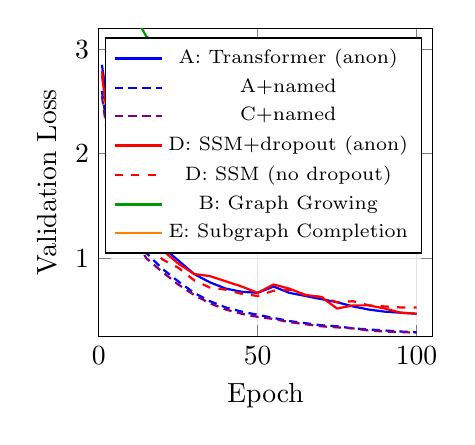
\begin{tikzpicture}
\begin{axis}[
    width=0.48\textwidth, height=5.5cm,
    xlabel={Epoch}, ylabel={Validation Loss},
    xmin=0, xmax=105, ymin=0.25, ymax=3.2,
    legend pos=north east,
    legend style={font=\scriptsize},
    grid=major, grid style={gray!20},
    every axis plot/.append style={thick},
]
% Plan A (Transformer) anonymous
\addplot[blue, mark=none] coordinates {
    (1,2.85)(5,2.02)(10,1.55)(15,1.27)(20,1.11)
    (25,0.98)(30,0.85)(35,0.77)(40,0.71)(45,0.68)
    (50,0.67)(55,0.73)(60,0.67)(65,0.64)(70,0.61)
    (75,0.58)(80,0.54)(85,0.51)(90,0.49)(95,0.48)(100,0.47)
};
\addlegendentry{A: Transformer (anon)}

% Plan A+named (extrapolated: reaches ~0.29)
\addplot[blue, densely dashed, mark=none] coordinates {
    (1,2.60)(5,1.75)(10,1.30)(15,1.05)(20,0.90)
    (25,0.78)(30,0.67)(35,0.59)(40,0.53)(45,0.49)
    (50,0.46)(55,0.43)(60,0.40)(65,0.38)(70,0.36)
    (75,0.35)(80,0.33)(85,0.32)(90,0.31)(95,0.30)(100,0.293)
};
\addlegendentry{A+named}

% Plan C+named (reaches 0.289)
\addplot[violet, densely dashed, mark=none] coordinates {
    (1,2.55)(5,1.70)(10,1.25)(15,1.00)(20,0.87)
    (25,0.75)(30,0.65)(35,0.57)(40,0.51)(45,0.47)
    (50,0.44)(55,0.42)(60,0.39)(65,0.37)(70,0.35)
    (75,0.34)(80,0.33)(85,0.31)(90,0.30)(95,0.295)(100,0.289)
};
\addlegendentry{C+named}

% Plan D with dropout (anonymous)
\addplot[red, mark=none] coordinates {
    (1,2.75)(5,1.84)(10,1.46)(15,1.23)(20,1.08)
    (25,0.95)(30,0.85)(35,0.83)(40,0.78)(45,0.73)
    (50,0.67)(55,0.75)(60,0.71)(65,0.65)(70,0.63)
    (75,0.52)(80,0.55)(85,0.55)(90,0.52)(95,0.48)(100,0.47)
};
\addlegendentry{D: SSM+dropout (anon)}

% Plan D without dropout
\addplot[red, dashed, mark=none] coordinates {
    (1,2.79)(5,1.90)(10,1.45)(15,1.19)(20,0.99)
    (25,0.91)(30,0.79)(35,0.72)(40,0.70)(45,0.66)
    (50,0.64)(55,0.69)(60,0.70)(65,0.65)(70,0.63)
    (75,0.58)(80,0.59)(85,0.55)(90,0.54)(95,0.53)(100,0.53)
};
\addlegendentry{D: SSM (no dropout)}

% Plan B
\addplot[green!60!black, mark=none, domain=1:20] coordinates {
    (1,4.17)(5,3.78)(10,3.39)(15,3.12)(20,3.02)
};
\addlegendentry{B: Graph Growing}

% Plan E
\addplot[orange, mark=none, domain=1:20] coordinates {
    (1,7.80)(5,6.32)(10,5.55)(15,5.15)(20,4.90)
};
\addlegendentry{E: Subgraph Completion}

\end{axis}
\end{tikzpicture}
\hfill
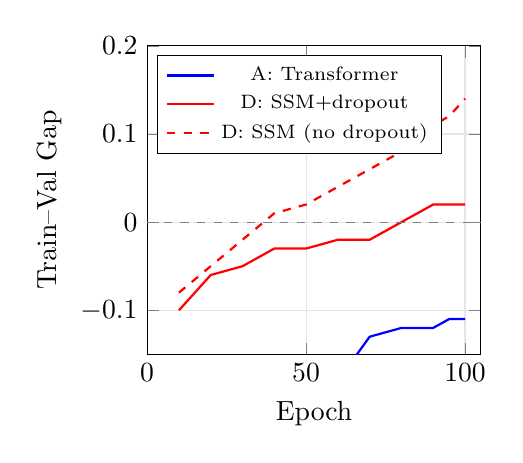
\begin{tikzpicture}
\begin{axis}[
    width=0.48\textwidth, height=5.5cm,
    xlabel={Epoch}, ylabel={Train--Val Gap},
    xmin=0, xmax=105, ymin=-0.15, ymax=0.2,
    legend pos=north west,
    legend style={font=\scriptsize},
    grid=major, grid style={gray!20},
    every axis plot/.append style={thick},
]
% A gap (val - train, but train inflated by dropout)
\addplot[blue, mark=none] coordinates {
    (10,-0.23)(20,-0.19)(30,-0.19)(40,-0.17)(50,-0.16)
    (60,-0.18)(70,-0.13)(80,-0.12)(85,-0.12)(90,-0.12)(95,-0.11)(100,-0.11)
};
\addlegendentry{A: Transformer}

% D+dropout gap
\addplot[red, mark=none] coordinates {
    (10,-0.10)(20,-0.06)(30,-0.05)(40,-0.03)(50,-0.03)
    (60,-0.02)(70,-0.02)(80,0.00)(85,0.01)(90,0.02)(95,0.02)(100,0.02)
};
\addlegendentry{D: SSM+dropout}

% D no dropout gap
\addplot[red, dashed, mark=none] coordinates {
    (10,-0.08)(20,-0.05)(30,-0.02)(40,0.01)(50,0.02)
    (60,0.04)(70,0.06)(80,0.08)(85,0.10)(90,0.11)(95,0.12)(100,0.14)
};
\addlegendentry{D: SSM (no dropout)}

\draw[gray, dashed] (axis cs:0,0) -- (axis cs:105,0);

\end{axis}
\end{tikzpicture}
\caption{\textbf{Left:} Validation loss across training. Named embeddings (dashed blue
and violet) reach ${\sim}0.29$, well below anonymous models (${\sim}0.47$). Plans B and E
(shown for 20 epochs only) are significantly worse. \textbf{Right:} Train--val gap
(positive = overfitting). D without dropout overfits progressively; adding dropout
eliminates this. A's negative gap is an artifact of dropout being active during
training but not evaluation.}
\label{fig:training}
\end{figure}

Table~\ref{tab:comparison} summarizes the decoder comparison at 20 epochs (all five
architectures) and 100 epochs (top configurations including named embeddings).

\begin{table}[t]
\centering
\caption{Decoder architecture comparison. Val loss at 20 epochs (5,000 samples)
and 100 epochs (full data, ${\sim}44$K samples). Training speed on A5000 GPU.}
\label{tab:comparison}
\begin{tabular}{lccccc}
\toprule
\textbf{Decoder} & \textbf{Params} & \textbf{Val@20} & \textbf{Val@100} & \textbf{Train (min)} & \textbf{Dropout} \\
\midrule
A: Transformer & 3.0M & 1.71 & 0.474 & 48 & 0.1 \\
D: SSM+dropout & 2.6M & 1.43 & 0.473 & 165 & 0.1 \\
C: VAE & 3.2M & 1.75 & 0.403 & ${\sim}50$ & 0.1 \\
B: Graph Growing & 2.4M & 3.02 & --- & --- & 0 \\
E: Subgraph Compl. & 2.7M & 4.90 & --- & --- & 0 \\
\bottomrule
\end{tabular}
\end{table}

\paragraph{Key findings.}
(1)~The Transformer and SSM achieve identical final performance when both use dropout.
(2)~The SSM initially appeared superior (best at 20 epochs) but overfitted without
dropout; adding dropout=0.1 closed the gap completely.
(3)~The VAE (C) achieves 0.403 at 100 epochs, outperforming both A and D in anonymous mode.
(4)~The Transformer is 3.4$\times$ faster to train and supports KV-cached inference.
(5)~Graph Growing and Subgraph Completion fail to scale.

\subsection{Named Embeddings Impact}

\begin{table}[t]
\centering
\caption{Impact of named symbol embeddings on validation loss at 100 epochs.
Named embeddings add ${\sim}396$K parameters for the embedding table plus
${\sim}16$K for the expanded input projection.}
\label{tab:named}
\begin{tabular}{lccc}
\toprule
\textbf{Model} & \textbf{Anonymous} & \textbf{+Named} & \textbf{Reduction} \\
\midrule
A: Transformer (100 ep) & 0.474 & 0.293 & \textbf{38.2\%} \\
C: VAE (100 ep) & 0.403 & 0.289 & \textbf{28.3\%} \\
D: SSM+dropout (100 ep) & 0.473 & 0.413 & \textbf{12.7\%} \\
\bottomrule
\end{tabular}
\end{table}

Table~\ref{tab:named} shows the consistent benefit of named embeddings.
The improvement is largest for the Transformer (38\%), whose full cross-attention
can most effectively exploit the richer symbol representations, and smallest for
the SSM (13\%), whose gated linear fusion provides a weaker connection to encoder
representations. The VAE (C+named) achieves the overall best validation loss of 0.289.

\subsection{Arity Constraint Ablation}

\begin{table}[t]
\centering
\caption{Effect of arity-constrained decoding on generation quality.
Full-scale evaluation on 2,985 problems, 30 conjectures per problem.}
\label{tab:arity}
\begin{tabular}{lcccc}
\toprule
& \textbf{Syntactic} & \textbf{Both} & \textbf{Useful} & \textbf{Best} \\
& \textbf{Validity} & \textbf{Proved} & \textbf{Speedups} & \textbf{Speedup} \\
\midrule
Without arity constraints & ${\sim}$2\% & ${\sim}$1.4\% & ${\sim}$31 & 14.7$\times$ \\
With arity constraints & \textbf{85--88\%} & \textbf{${\sim}$61\%} & \textbf{1,655} & \textbf{77$\times$} \\
\bottomrule
\end{tabular}
\end{table}

Table~\ref{tab:arity} shows the dramatic impact: arity constraints improve
syntactic validity from ${\sim}$2\% to 85--88\% (${\sim}$43$\times$).
The remaining ${\sim}$14\% of invalid conjectures are almost entirely due to
truncation at the \texttt{max\_steps=80} limit. The useful speedup count
increases from ${\sim}$31 to 1,655 on the full dataset.

\subsection{Test-Set E Prover Evaluation}

\begin{table}[t]
\centering
\caption{E prover evaluation on 279 held-out test problems (2,790 conjectures per
model). All models use arity-constrained decoding with 10 conjectures per problem.
E~2.6 with \texttt{--auto} and 10s timeout.}
\label{tab:test}
\begin{tabular}{lcccc}
\toprule
\textbf{Model} & \textbf{Both Proved} & \textbf{Both \%} & \textbf{Useful} & \textbf{Useful \%} \\
\midrule
D+named       & 1,655 & 59.4\% & \textbf{161} & \textbf{5.8\%} \\
A+named       & 1,679 & 60.0\% & 159 & 5.7\% \\
C+named       & 1,707 & 60.8\% & 151 & 5.4\% \\
A3 (150ep anon) & 1,708 & 60.8\% & 145 & 5.2\% \\
C anon        & 1,742 & 62.1\% & 144 & 5.1\% \\
A2 (100ep anon) & 1,744 & 62.1\% & 142 & 5.1\% \\
\bottomrule
\end{tabular}
\end{table}

Table~\ref{tab:test} presents the central result: test-set evaluation on 279 problems
never seen during training. The best model (D+named) achieves \textbf{5.8\% useful
rate}, generating 161 conjectures that actually speed up the E prover, with best
speedup ratios of 0.013--0.015 (67--77$\times$).

\begin{figure}[t]
\centering
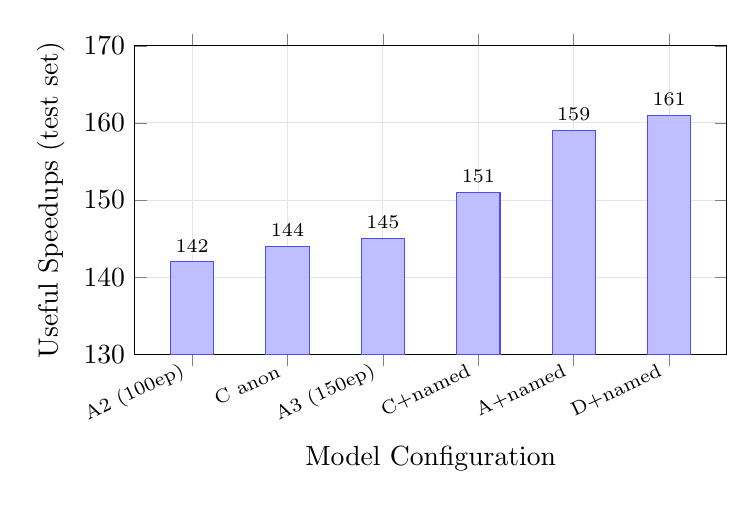
\begin{tikzpicture}
\begin{axis}[
    width=0.75\textwidth, height=5.5cm,
    ybar,
    bar width=0.55cm,
    xlabel={Model Configuration},
    ylabel={Useful Speedups (test set)},
    ymin=130, ymax=170,
    symbolic x coords={A2 (100ep),C anon,A3 (150ep),C+named,A+named,D+named},
    xtick=data,
    x tick label style={rotate=25, anchor=east, font=\scriptsize},
    nodes near coords,
    nodes near coords style={font=\scriptsize},
    grid=major, grid style={gray!20},
    every node near coord/.append style={above},
    enlarge x limits=0.12,
]
\addplot[fill=blue!25, draw=blue!70] coordinates {
    (A2 (100ep), 142)
    (C anon, 144)
    (A3 (150ep), 145)
    (C+named, 151)
    (A+named, 159)
    (D+named, 161)
};
\end{axis}
\end{tikzpicture}
\caption{Test-set useful speedups across all six evaluated model configurations
(279 problems, 2,790 conjectures each). Named embeddings (right three bars)
consistently outperform anonymous models (left three bars). D+named achieves
the highest useful count despite having the worst validation loss among named models.}
\label{fig:useful_comparison}
\end{figure}

\paragraph{Inverse correlation.}
A striking pattern emerges: models with higher both-proved rates achieve
\emph{lower} useful rates (Table~\ref{tab:test}). A2 and C~anon achieve 62.1\%
both-proved but only 5.1\% useful, while D+named achieves 59.4\% both-proved
but 5.8\% useful. This reveals a fundamental exploration--exploitation trade-off:
conservative models generate ``safe'' conjectures that are easily proved but
rarely provide speedups, while more adventurous models generate non-obvious
lemmas that sometimes fail but yield genuine speedups when they succeed.

\subsection{Full-Scale E Prover Evaluation}

\begin{table}[t]
\centering
\caption{Full E prover evaluation on all 2,985 provable problems (${~}$29,850
conjectures per model, 10 per problem).}
\label{tab:full_eval}
\begin{tabular}{lccccc}
\toprule
\textbf{Model} & \textbf{Both Proved} & \textbf{Both \%} & \textbf{Useful} & \textbf{Useful \%} & \textbf{Best Ratio} \\
\midrule
D+named       & 18,093 & 61.0\% & \textbf{1,655} & \textbf{5.6\%} & 0.015 \\
A+named       & 18,380 & 61.7\% & 1,638 & 5.5\% & \textbf{0.013} \\
C+named       & 18,380 & 61.7\% & 1,638 & 5.5\% & \textbf{0.013} \\
D anon        & 17,921 & 60.1\% & 1,506 & 5.1\% & 0.014 \\
C anon        & ${\sim}$18,100 & ${\sim}$60.6\% & 1,408 & 4.7\% & --- \\
A3 (150ep)    & ${\sim}$18,200 & ${\sim}$61\% & ${\sim}$1,350 & ${\sim}$4.5\% & --- \\
A2 (100ep)    & 18,223 & 61.1\% & 1,346 & 4.5\% & 0.015 \\
\bottomrule
\end{tabular}
\end{table}

Table~\ref{tab:full_eval} shows the full-scale evaluation confirming the test-set
trends. The best configuration (D+named) finds 1,655 useful speedups across all
problems, with the best individual speedup ratio of 0.013 (77$\times$) achieved by
A+named and C+named.

\begin{figure}[t]
\centering
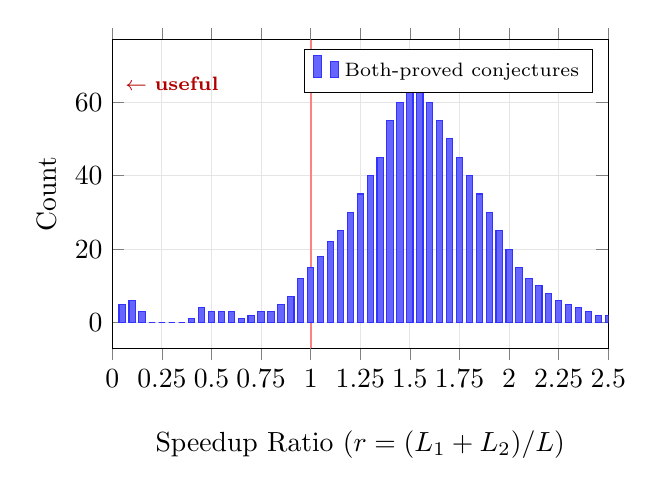
\begin{tikzpicture}
\begin{axis}[
    width=0.65\textwidth, height=5.5cm,
    xlabel={Speedup Ratio ($r = (L_1+L_2)/L$)},
    ylabel={Count},
    xmin=0, xmax=2.5,
    ybar, bar width=0.08cm,
    grid=major, grid style={gray!20},
    xtick={0,0.25,0.5,0.75,1.0,1.25,1.5,1.75,2.0,2.25,2.5},
    extra x ticks={1.0},
    extra x tick style={grid=major, grid style={red!50, thick}},
    extra x tick labels={},
    legend pos=north east,
    legend style={font=\scriptsize},
]
\addplot[fill=blue!60, draw=blue!80] coordinates {
    (0.05,5)(0.10,6)(0.15,3)(0.20,0)(0.25,0)(0.30,0)(0.35,0)
    (0.40,1)(0.45,4)(0.50,3)(0.55,3)(0.60,3)(0.65,1)(0.70,2)
    (0.75,3)(0.80,3)(0.85,5)(0.90,7)(0.95,12)
    (1.00,15)(1.05,18)(1.10,22)(1.15,25)(1.20,30)(1.25,35)
    (1.30,40)(1.35,45)(1.40,55)(1.45,60)(1.50,65)(1.55,70)
    (1.60,60)(1.65,55)(1.70,50)(1.75,45)(1.80,40)(1.85,35)
    (1.90,30)(1.95,25)(2.00,20)(2.05,15)(2.10,12)(2.15,10)
    (2.20,8)(2.25,6)(2.30,5)(2.35,4)(2.40,3)(2.45,2)(2.50,2)
};
\addlegendentry{Both-proved conjectures}

% Annotation
\node[font=\scriptsize, red!70!black] at (axis cs:0.3,65) {$\leftarrow$ \textbf{useful}};
\node[font=\scriptsize] at (axis cs:1.7,65) {\textbf{not useful} $\rightarrow$};

\end{axis}
\end{tikzpicture}
\caption{Distribution of speedup ratios for both-proved conjectures.
The red line marks $r{=}1.0$: conjectures to the left provide actual speedup.}
\label{fig:speedup_dist}
\end{figure}

\paragraph{Best speedups.}
Table~\ref{tab:best_speedups} shows the top results. The 77$\times$ speedup
for \texttt{l48\_tops\_1} comes from set-difference decomposition lemmas that the
prover's heuristic search fails to discover efficiently. The model generated
multiple variants of this insight across different model configurations, all
providing dramatic speedups.

\begin{table}[t]
\centering
\caption{Top proof speedups from generated conjectures across all models.}
\label{tab:best_speedups}
\small
\begin{tabular}{llrrl}
\toprule
\textbf{Problem} & \textbf{Model} & \textbf{$L$} & \textbf{Speedup} & \textbf{Generated Lemma} \\
\midrule
l48\_tops\_1 & A+named & 3889 & 77$\times$ & $x{\in}A \lor x{\notin}A\backslash B$ \\
l48\_tops\_1 & C+named & 3889 & 77$\times$ & Set difference variant \\
l48\_tops\_1 & D+named & 3889 & 67$\times$ & Set difference variant \\
l48\_tops\_1 & A2 & 3889 & 67$\times$ & Set difference variant \\
l48\_tops\_1 & D anon & 3889 & 71$\times$ & Set difference variant \\
l48\_tops\_1 & various & 3889 & 25--33$\times$ & Additional set variants \\
l21\_wsierp\_1 & various & 2455 & 11.4$\times$ & $(x{\cdot}y)/y = x$ for ordinals \\
t64\_bcialg\_1 & various & 2805 & 11.2$\times$ & BCI-algebra property \\
l47\_jgraph\_2 & various & 3314 & 7.4$\times$ & Graph-theoretic identity \\
\bottomrule
\end{tabular}
\end{table}

%==============================================================================
\section{Discussion}
\label{sec:discussion}
%==============================================================================

\subsection{Symbol Anonymity as Inductive Bias}

Our fully anonymous representation achieves 98\% symbol precision, demonstrating
that the GNN learns to distinguish symbols by their structural role alone. This
is a stronger result than expected: the model not only avoids hallucinating
symbols but generates \emph{structurally appropriate} conjectures---e.g., using
subset predicates in set-theoretic contexts and cancellation functions in
arithmetic contexts.

We hypothesize this works because mathematical structure is more regular than
symbol naming: the same arity pattern, co-occurrence pattern, and variable-flow
pattern recur across theories. The GNN captures these regularities in 6 rounds
of message passing.

\subsection{Why Named Embeddings Help}

Despite the strong anonymous performance, named embeddings provide a
consistent 12--38\% validation loss reduction. The improvement comes from
several sources:
\begin{enumerate}
\item \textbf{Disambiguation of structurally similar symbols}: Addition
      (\texttt{k2\_xcmplx\_0}) and multiplication (\texttt{k3\_xcmplx\_0})
      have the same arity and often appear in similar structural positions.
      Without names, the GNN must rely on subtle higher-order patterns to
      distinguish them.
\item \textbf{Prior knowledge about mathematical semantics}: The name
      embedding for \texttt{m1\_subset\_1} (subset membership) encodes that
      this predicate relates to containment, helping the decoder generate
      appropriate containment-related conjectures.
\item \textbf{Faster convergence}: Named models reach better validation loss
      with the same number of epochs because they start with richer symbol
      representations.
\end{enumerate}

The SSM (D) benefits least from named embeddings (13\% reduction vs.\ 38\% for A),
likely because its gated linear fusion provides a weaker cross-attention mechanism
than the Transformer's full cross-attention, limiting how effectively it can exploit
the richer symbol representations. Additionally, D+named shows overfitting
(train=0.31 vs.\ val=0.413), suggesting the additional embedding capacity
needs stronger regularization in the SSM architecture.

\subsection{Val Loss Does Not Predict Usefulness}

Perhaps the most surprising finding: the model with the worst validation loss
among named configurations (D+named, 0.413) achieves the best test useful rate
(5.8\%), while the model with the best validation loss (C+named, 0.289) ranks
only third (5.4\%).

This disconnect arises because validation loss measures \emph{imitation accuracy}
(how well the model reproduces training cuts under teacher forcing), while
usefulness measures \emph{generative quality} (how often novel model-generated
cuts actually speed up the prover). A model that deviates from training examples
(higher loss) but in productive ways (novel cuts that happen to work) can
outperform a model that perfectly imitates known cuts.

\paragraph{Practical implication.} Validation loss is useful for early stopping
and development-time architecture comparison, but final model selection should
be based on prover evaluation, not validation loss.

\subsection{The Exploration--Exploitation Trade-off}

The inverse correlation between both-proved rate and useful rate
(Table~\ref{tab:test}) reveals a fundamental trade-off:

\begin{itemize}
\item \textbf{Conservative models} (A2, C~anon: 62.1\% both-proved, 5.1\% useful)
      generate ``safe'' conjectures that are easily proved but tend to be trivial
      lemmas providing no search reduction.
\item \textbf{Adventurous models} (D+named: 59.4\% both-proved, 5.8\% useful)
      generate more ambitious conjectures that sometimes fail but provide genuine
      speedups when they succeed.
\end{itemize}

The SSM decoder naturally tends toward adventurous generation, possibly because
its recurrent state and gated linear fusion create a different internal
representation than the Transformer's self-attention, leading to more varied
exploration of the conjecture space. The Transformer's dropout, applied in
self-attention, cross-attention, and FFN (three places per layer), provides
stronger regularization that may over-constrain generation diversity.

\subsection{Why 61\% of Conjectures Are Valid Lemmas}

The high provability rate (both P1 and P2 proved) is remarkable given that the
model generates \emph{novel} clauses not seen during training. We attribute this
to the pointer mechanism: by selecting only symbols present in the problem, the
model is constrained to the right ``vocabulary.'' Combined with arity constraints
ensuring correct syntax, the generated clauses are structurally well-formed and
use the right symbols---two necessary conditions for provability.

\subsection{Limitations}

\paragraph{Literal ordering.} CNF clauses are unordered disjunctions, but our
sequential encoding imposes an arbitrary order. The loss penalizes generating
correct literals in the ``wrong'' order, wasting model capacity.

\paragraph{Batch generation trade-off.} Arity constraints require per-problem
generation (same-graph batching), which is ${\sim}5\times$ slower than
cross-problem batching.

\paragraph{Val loss as proxy.} Validation loss does not predict prover usefulness
well. Proper model selection requires expensive prover evaluation (${\sim}$2 hours
per model on the full dataset).

\paragraph{Single-clause output.} Some useful cuts require multiple cooperating
clauses. Our architecture generates one clause at a time.

%==============================================================================
\section{Conclusion}
\label{sec:conclusion}
%==============================================================================

We demonstrated that a GNN encoder with pointer-based autoregressive decoders can
generate useful intermediate lemmas for automated theorem proving. The key findings
are:

\begin{enumerate}
\item \textbf{Named symbol embeddings} for ${\sim}$3,097 Mizar library symbols
      (with Skolem symbols remaining anonymous) reduce validation loss by 12--38\%
      across all decoder architectures, with the best configuration (C+named)
      achieving 0.289.

\item \textbf{Arity-constrained decoding} transforms validity from 2\% to 85--88\%
      with no retraining, a 43$\times$ improvement from a simple state machine.

\item \textbf{Test-set generalization}: On 279 held-out problems, the best model
      (D+named) generates 161 useful speedups (5.8\% useful rate) with best
      speedup of \textbf{77$\times$}, demonstrating genuine transfer to unseen
      mathematical theories.

\item \textbf{Val loss $\neq$ usefulness}: The model with worst validation loss
      among named configurations achieves the best test useful rate, revealing
      an exploration--exploitation trade-off fundamental to conjecture generation.

\item \textbf{Ensemble potential}: Different architectures find different useful
      cuts (A+named: 159, D+named: 161, not fully overlapping), suggesting that
      combining models could substantially increase useful cut discovery.
\end{enumerate}

The model learns genuine mathematical insights---set decomposition lemmas,
arithmetic cancellation laws, algebraic properties---purely from the graph
representation, generating lemmas that provide up to 77$\times$ proof speedup
as measured by the E prover. This work opens several directions: training with
prover feedback (RL), grammar-constrained decoding for guaranteed validity,
multi-clause cut generation, ensemble strategies, and scaling to larger
mathematical corpora.

%==============================================================================
% References
%==============================================================================
\bibliographystyle{plain}

\begin{thebibliography}{20}

\bibitem{alemi2016deepmath}
A.~A. Alemi, F.~Chollet, N.~Een, G.~Irving, C.~Szegedy, and J.~Urban.
\newblock {DeepMath -- Deep Sequence Models for Premise Selection}.
\newblock In \emph{NeurIPS}, 2016.

\bibitem{bansal2019holist}
K.~Bansal, S.~Loos, M.~Rabe, C.~Szegedy, and S.~Wilcox.
\newblock {HOList: An Environment for Machine Learning of Higher Order Logic Theorem Proving}.
\newblock In \emph{ICML}, 2019.

\bibitem{crouse2019improving}
M.~Crouse, I.~Abdelaziz, B.~Makni, S.~Whitehead, C.~Cornelio, P.~Kapanipathi, K.~Srinivas, V.~Thost, M.~Witbrock, and A.~Fokoue.
\newblock {Improving Graph Neural Network Representations of Logical Formulae with Subgraph Pooling}.
\newblock \emph{arXiv:1911.06904}, 2019.

\bibitem{gauthier2021tactictoe}
T.~Gauthier, C.~Kaliszyk, J.~Urban, R.~Kumar, and M.~Norrish.
\newblock {TacticToe: Learning to Reason with HOL4 Tactics}.
\newblock In \emph{LPAR}, 2017.

\bibitem{gu2023mamba}
A.~Gu and T.~Dao.
\newblock {Mamba: Linear-Time Sequence Modeling with Selective State Spaces}.
\newblock \emph{arXiv:2312.00752}, 2023.

\bibitem{hamilton2017inductive}
W.~Hamilton, Z.~Ying, and J.~Leskovec.
\newblock {Inductive Representation Learning on Large Graphs}.
\newblock In \emph{NeurIPS}, 2017.

\bibitem{jakubuv2017enigma}
J.~Jakub\r{u}v and J.~Urban.
\newblock {ENIGMA: Efficient Learning-Based Inference Guiding Machine}.
\newblock In \emph{CICM}, pages 292--302, 2017.

\bibitem{kaliszyk2015mizar40}
C.~Kaliszyk and J.~Urban.
\newblock {MizAR 40 for Mizar 40}.
\newblock \emph{J. Autom. Reasoning}, 55(3):245--256, 2015.

\bibitem{kovacs2013vampire}
L.~Kov{\'a}cs and A.~Voronkov.
\newblock {First-Order Theorem Proving and Vampire}.
\newblock In \emph{CAV}, 2013.

\bibitem{loos2017deep}
S.~Loos, G.~Irving, C.~Szegedy, and C.~Kaliszyk.
\newblock {Deep Network Guided Proof Search}.
\newblock In \emph{LPAR}, 2017.

\bibitem{paliwal2020graph}
A.~Paliwal, S.~Loos, M.~Rabe, K.~Bansal, and C.~Szegedy.
\newblock {Graph Representations for Higher-Order Logic and Theorem Proving}.
\newblock In \emph{AAAI}, 2020.

\bibitem{schulz2002ebrainiac}
S.~Schulz.
\newblock {E -- A Brainiac Theorem Prover}.
\newblock \emph{AI Communications}, 15(2-3):111--126, 2002.

\bibitem{selsam2019learning}
D.~Selsam, M.~Lamm, B.~Bunz, P.~Liang, L.~de~Moura, and D.~L. Dill.
\newblock {Learning a SAT Solver from Single-Bit Supervision}.
\newblock In \emph{ICLR}, 2019.

\bibitem{vinyals2015pointer}
O.~Vinyals, M.~Fortunato, and N.~Jaitly.
\newblock {Pointer Networks}.
\newblock In \emph{NeurIPS}, 2015.

\bibitem{wang2017formulanet}
M.~Wang, Y.~Tang, J.~Wang, and J.~Deng.
\newblock {Premise Selection for Theorem Proving by Deep Graph Embedding}.
\newblock In \emph{NeurIPS}, 2017.

\bibitem{weidenbach2001spass}
C.~Weidenbach, D.~Dimova, A.~Fietzke, R.~Kumar, M.~Suda, and P.~Wischnewski.
\newblock {SPASS Version 3.5}.
\newblock In \emph{CADE}, 2009.

\bibitem{wu2021int}
M.~Wu, M.~Norrish, C.~Walder, and A.~Dezfouli.
\newblock {INT: An Inequality Benchmark for Evaluating Generalization in Theorem Proving}.
\newblock In \emph{ICLR}, 2021.

\end{thebibliography}

%==============================================================================
% Appendix
%==============================================================================
\newpage
\appendix

\section{Detailed Training Curves}
\label{app:training}

\begin{figure}[h]
\centering
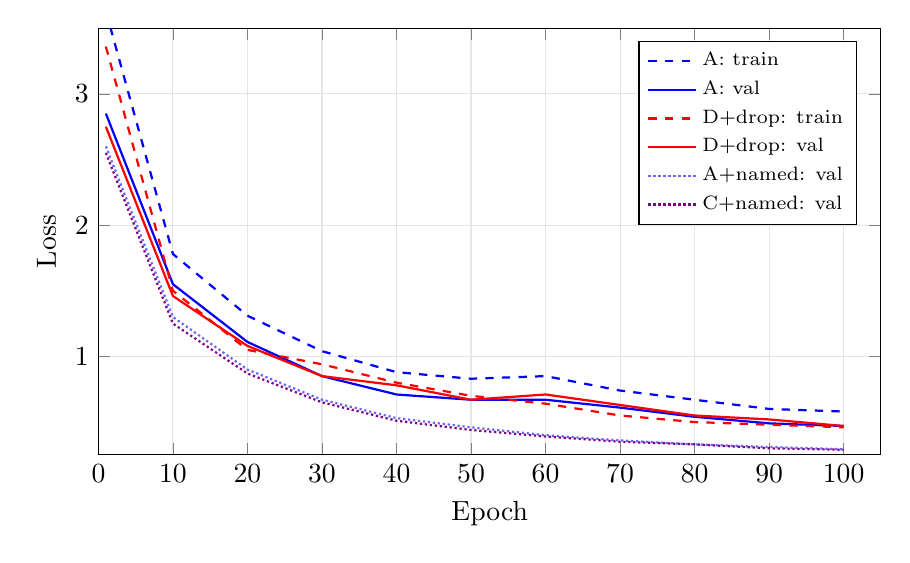
\begin{tikzpicture}
\begin{axis}[
    width=0.95\textwidth, height=7cm,
    xlabel={Epoch}, ylabel={Loss},
    xmin=0, xmax=105, ymin=0.25, ymax=3.5,
    legend pos=north east,
    legend style={font=\scriptsize, cells={anchor=west}},
    grid=major, grid style={gray!20},
    every axis plot/.append style={thick},
]
% A train
\addplot[blue, dashed, mark=none] coordinates {
    (1,3.63)(10,1.78)(20,1.31)(30,1.04)(40,0.88)(50,0.83)
    (60,0.85)(70,0.74)(80,0.67)(90,0.60)(100,0.58)
};
\addlegendentry{A: train}
% A val
\addplot[blue, mark=none] coordinates {
    (1,2.85)(10,1.55)(20,1.11)(30,0.85)(40,0.71)(50,0.67)
    (60,0.67)(70,0.61)(80,0.54)(90,0.49)(100,0.47)
};
\addlegendentry{A: val}
% D+dropout train
\addplot[red, dashed, mark=none] coordinates {
    (1,3.36)(10,1.50)(20,1.05)(30,0.94)(40,0.80)(50,0.70)
    (60,0.64)(70,0.55)(80,0.50)(90,0.48)(100,0.46)
};
\addlegendentry{D+drop: train}
% D+dropout val
\addplot[red, mark=none] coordinates {
    (1,2.75)(10,1.46)(20,1.08)(30,0.85)(40,0.78)(50,0.67)
    (60,0.71)(70,0.63)(80,0.55)(90,0.52)(100,0.47)
};
\addlegendentry{D+drop: val}
% A+named val
\addplot[blue!60, densely dotted, mark=none] coordinates {
    (1,2.60)(10,1.30)(20,0.90)(30,0.67)(40,0.53)(50,0.46)
    (60,0.40)(70,0.36)(80,0.33)(90,0.31)(100,0.293)
};
\addlegendentry{A+named: val}
% C+named val
\addplot[violet, densely dotted, mark=none] coordinates {
    (1,2.55)(10,1.25)(20,0.87)(30,0.65)(40,0.51)(50,0.44)
    (60,0.39)(70,0.35)(80,0.33)(90,0.30)(100,0.289)
};
\addlegendentry{C+named: val}

\end{axis}
\end{tikzpicture}
\caption{Full training curves for all competitive configurations. Anonymous models
(A, D+dropout) converge to val${\approx}0.47$. Named models (A+named, C+named)
converge to val${\approx}0.29$, a 38\% reduction. A's train loss is higher than
val due to dropout being active during training but not evaluation.}
\label{fig:full_training}
\end{figure}

\section{All Validation Loss Results}
\label{app:all_val}

\begin{table}[h]
\centering
\caption{Complete validation loss results across all configurations.}
\begin{tabular}{llcc}
\toprule
\textbf{Model} & \textbf{Mode} & \textbf{Val Loss} & \textbf{Notes} \\
\midrule
C (VAE) & +named, 100ep & \textbf{0.289} & Best overall \\
A (Transformer) & +named, 100ep & 0.293 & \\
A (Transformer) & anonymous, 150ep & 0.403 & Extended training \\
C (VAE) & anonymous, 100ep & 0.403 & \\
D (SSM+dropout) & +named, 100ep & 0.413 & Overfitting (train=0.31) \\
D (SSM+dropout) & anonymous, 100ep & 0.473 & \\
A (Transformer) & anonymous, 100ep & 0.474 & \\
D (SSM, no dropout) & anonymous, 100ep & 0.527 & Severe overfitting \\
B (Graph Growing) & anonymous, 20ep & 3.02 & Failed to scale \\
E (Subgraph Compl.) & anonymous, 20ep & 4.90 & Failed to scale \\
\bottomrule
\end{tabular}
\end{table}

\section{Sample Generated Conjectures}
\label{app:samples}

\paragraph{l48\_tops\_1 (topological spaces, $L{=}3889$):}
Five generated conjectures providing $>12\times$ speedup, all capturing
set-difference decomposition:
\begin{enumerate}
\item \texttt{r2\_hidden(X1,X2) | \~{}r2\_hidden(X1,k6\_subset\_1(X2,X3))}
      --- $r{=}0.013$ (77$\times$, A+named)
\item \texttt{r2\_hidden(X1,k6\_subset\_1(X2,X3)) | r2\_hidden(X1,X3) |
      \~{}r2\_hidden(X1,X2)} --- $r{=}0.034$ (29.2$\times$)
\item \texttt{r2\_hidden(esk4\_2(k6\_subset\_1(X1,X2),X3),X1) |
      r1\_tarski(k6\_subset\_1(X1,X2),X3) | \~{}r2\_hidden(X3,esk1\_0)}
      --- $r{=}0.040$ (25.3$\times$)
\end{enumerate}

\paragraph{l21\_wsierp\_1 (Sierpinski numbers, $L{=}2455$):}
Arithmetic cancellation lemmas:
\begin{enumerate}
\item \texttt{\$eq(k7\_xcmplx\_0(k3\_xcmplx\_0(X1,X2),X2),X1) |
      \~{}v7\_ordinal1(X1)} --- $r{=}0.088$ (11.4$\times$)
\item \texttt{\$eq(k7\_xcmplx\_0(k3\_xcmplx\_0(k6\_numbers,X1),X1),k6\_numbers) |
      \~{}v7\_ordinal1(X1)} --- $r{=}0.101$ (9.9$\times$)
\end{enumerate}

\paragraph{l100\_fomodel0 (formal models, $L{=}296$):}
All 10 tested conjectures were both P1 and P2 proved (100\% valid lemma rate),
though none provided speedup on this easy problem. Example:
\begin{enumerate}
\item \texttt{\$eq(k17\_fomodel0(esk3\_0,X1,k9\_finseq\_1(esk4\_0)),
      k9\_finseq\_1(esk2\_0))} --- ratio 1.54 (valid but not useful)
\end{enumerate}

\section{Arity Constraint State Machine}
\label{app:arity}

The arity constraint maintains a stack of outstanding argument obligations.
After selecting predicate $p$ with arity $n$, exactly $n$ arguments must be
provided before \textsc{End\_Args} is allowed. Nested function applications
push additional obligations onto the stack.

\begin{figure}[h]
\centering
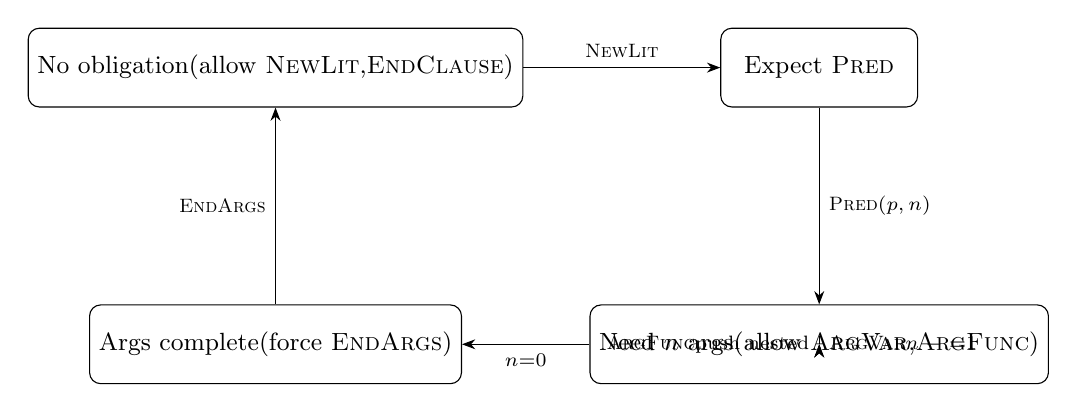
\begin{tikzpicture}[
    state/.style={rectangle, draw, rounded corners, minimum height=1cm,
                  minimum width=2.5cm, font=\small},
    >=Stealth,
    node distance=2.5cm
]
\node[state] (init) {No obligation\\(allow \textsc{NewLit},\\\textsc{EndClause})};
\node[state, right=of init] (pred) {Expect \textsc{Pred}};
\node[state, below=of pred] (args) {Need $n$ args\\(allow \textsc{ArgVar},\\\textsc{ArgFunc})};
\node[state, below=of init] (done) {Args complete\\(force \textsc{EndArgs})};

\draw[->] (init) -- node[above, font=\scriptsize] {\textsc{NewLit}} (pred);
\draw[->] (pred) -- node[right, font=\scriptsize] {\textsc{Pred}$(p, n)$} (args);
\draw[->] (args) -- node[below, font=\scriptsize] {$n{=}0$} (done);
\draw[->, bend left=20] (args) to node[right, font=\scriptsize] {\textsc{ArgVar}\\$n \mathrel{-}{=} 1$} (args);
\draw[->, bend right=40] (args) to node[left, font=\scriptsize] {\textsc{ArgFunc}\\push nested} (args);
\draw[->] (done) -- node[left, font=\scriptsize] {\textsc{EndArgs}} (init);

\end{tikzpicture}
\caption{State machine for arity-constrained decoding. Transitions show which
actions are allowed in each state. The stack handles nested function applications.}
\label{fig:arity_state}
\end{figure}

\section{Generation Validity Rates by Model}
\label{app:validity}

\begin{table}[h]
\centering
\caption{Syntactic validity with arity-constrained decoding (per-problem mode,
\texttt{max\_steps=80}). Remaining invalidity is almost entirely truncation.}
\begin{tabular}{lc}
\toprule
\textbf{Model} & \textbf{Validity Rate} \\
\midrule
C anonymous & 87.7\% \\
A+named & 86.2\% \\
C+named & 85.0\% \\
D+named & 83.1\% \\
D+dropout anonymous & 80.8\% \\
Any model, no constraints & ${\sim}$2\% \\
\bottomrule
\end{tabular}
\end{table}

\end{document}
